\subsection{Systemanalyse und -entwurf}

Aufbauend auf die Anforderung, einen Prototypen mit den Technologien der SAP Leonardo IoT Foundation zu entwickeln, wird in diesem Kapitel die zugrundeliegende Systemarchitektur untersucht. Dabei erfüllt die Analyse mehrere Zwecke. Zum einen wird die Forschungsfrage FF-1.2 (s. \ref{problemstellung}), welche Möglichkeiten zur intelligenten Vernetzung die Architektur bietet, beantwortet. An die Beantwortung dieser Frage knüpft sich die Prüfung der Kompatibilität der Zielarchitektur mit der \ac{rami}. In der Anforderungsanalyse wurde hauptsächlich die Anwendung des cloud-basierten Ansatzes als Lösung (s. \ref{technischeraufbau}) spezifiziert. Aus diesem Grund wird auf Grundlage der Analyse die angepasste Architektur des Zielsystems als Lösung für den technischen Aufbau entworfen.

\subsubsection{Systemarchitektur}

Wie in Abschnitt \ref{leo} beschrieben, bietet die SAP Leonardo IoT Foundation zahlreiche Dienste zur Integration von physischen Geräten in die SAP Cloud Platform. Die Abbildung \ref{saparch} zeigt den typischen Verlauf eines solchen Integrationsprozesses. Die realen Geräte senden ihre Daten über \textit{Gateways} an die \textit{SAP Cloud Platform Internet of Things Services} (1). Dort werden sie in einer PostgreSQL Datenbank gehalten \citep{Acharya2019}. Der Zugriff auf die Daten der \ac{cpss} erfolgt im Rahmen einer \acf{soa} über verschiedene \ac{api}. Um die Geräte in eine IoT-Anwendung zu integrieren, werden sie via \textit{Message Processing} and das \textit{IoT Application Enablement} gesendet (2). Dort können digitale Zwillinge und ihre Funktionen definiert werden. Für die Anwendungsentwicklung werden die Daten per OData oder REST-Schnittstellen von der Cloud Foundry Umgebung an die WebIDE in der Neo Umgebung übergeben (3). Anschließend wird die Anwendung in die Cloud Foundry deployed. Die einzelnen Komponenten und Konzepte werden im Folgenden näher im Detail erläutert.



\begin{figure}[ht!]
  \centering
  \noindent\makebox[\textwidth]{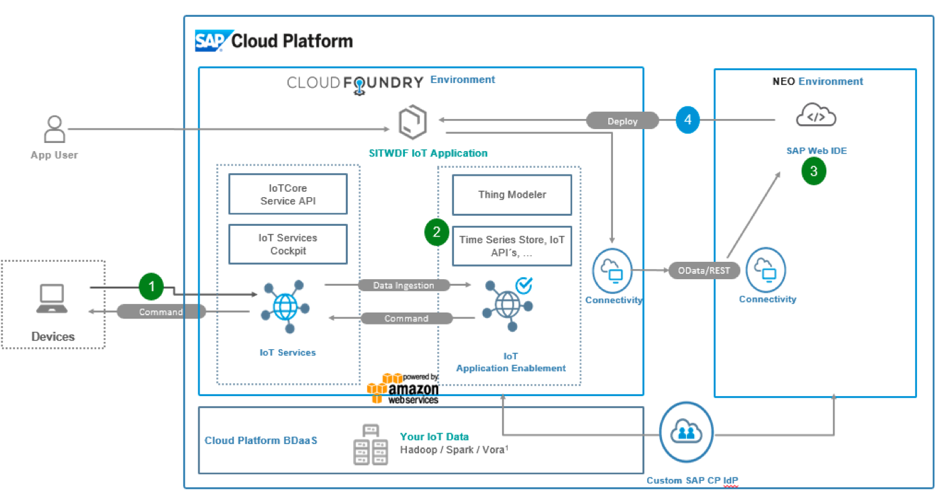
\includegraphics[width=\paperwidth]{sap_architecture.png}}
  \caption[Architektur von SAP]{Architektur von SAP \citep{Ganz2019}}
  \label{saparch}
\end{figure}

\subsubsection{SCP Internet of Things Services}

\begin{figure}[H]
  \centering
  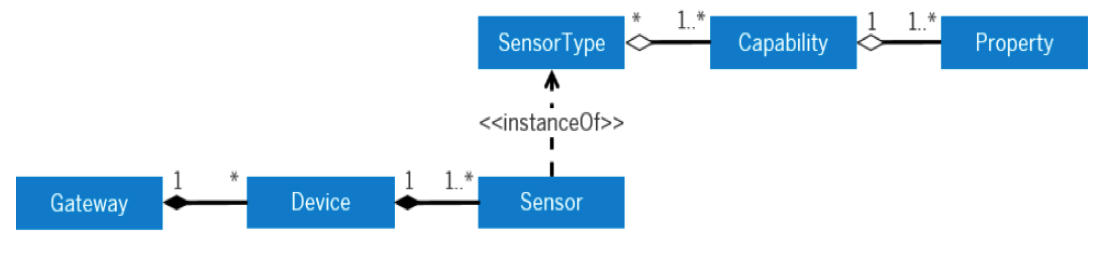
\includegraphics[width=1.0\linewidth]{pictures/device_model}
  \caption[Gerätemodell]{Gerätemodell}
  \label{fig:filename_without_extension}
\end{figure}

\subsubsection{Einheitliche Kommunikation: REST API}

\subsubsection{Edge-Processing}

Protokolle der Edge Server CoAP, File, Modbus, MQTT, OPC UA, REST, SigFox, SNMP
\subsubsection{Destinations}
Destinations: Warum braucht man Destinations und welche man benötigt (SNS),  wenn man kommunizieren will mit
Externe Services wie AWS SNS
Interne Kommunikation der SCP CF und NEO
Communication zwischen Cloud Services AWS SNS und SAP Leonardo

\subsubsection{Message Processing}
Leonardo IoT, SQL Kafka: Ich hab Leonardo IoT benutzt (in prototype erwähnen)

\subsubsection{SAP Leonardo Application Enablement}
Für die Integration der Geräte in Anwendungen werden hier digitale Zwllinge erstellt
Thing Modeler und freestyle IoT Applications
\subsubsection{Sicherheit}
OAuth, SSL/TLS, SAML 2.0: erklären, was SAP und AWS auch eventuell haben

\subsubsection{Kompatibiliät mit Referenzarchitektur}

\begin{figure}[H]
  \centering
  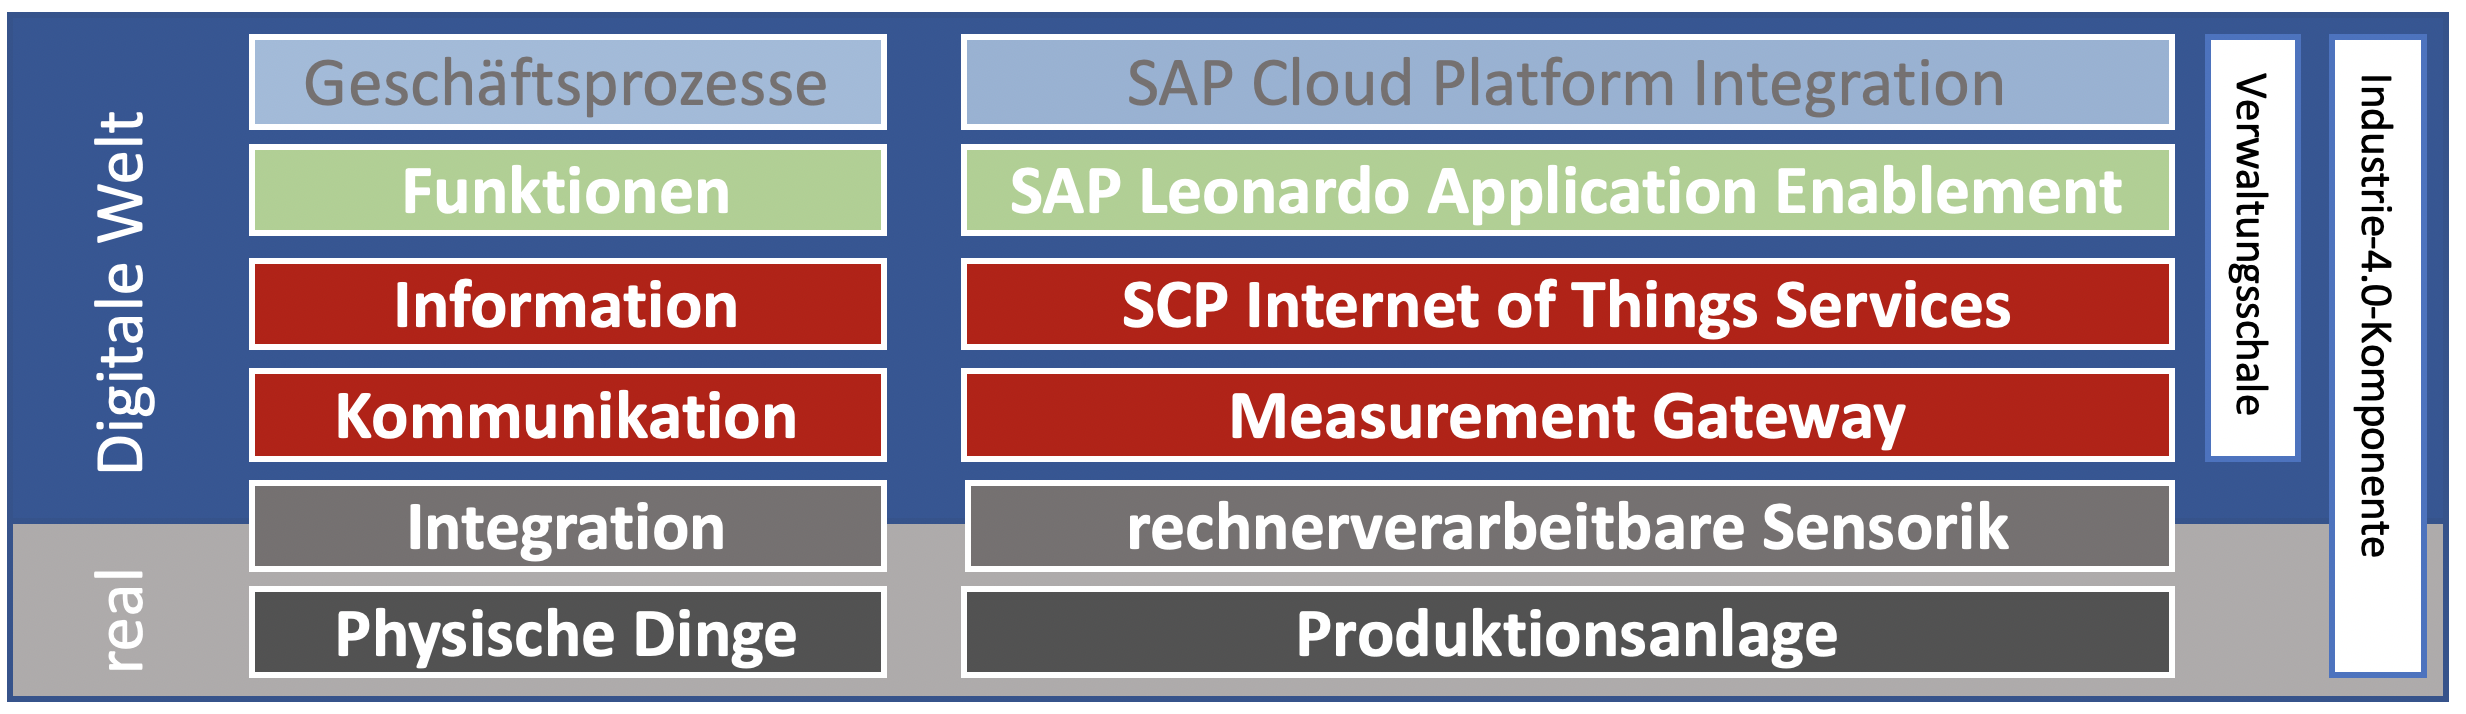
\includegraphics[width=1.0\linewidth]{pictures/rami_custom1}
  \caption[Referenz zu den Schichten der RAMI 4.0]{Referenz zu den Schichten der RAMI 4.0}
  \label{ramicustom}
\end{figure}

\begin{figure}[h]
  \centering
  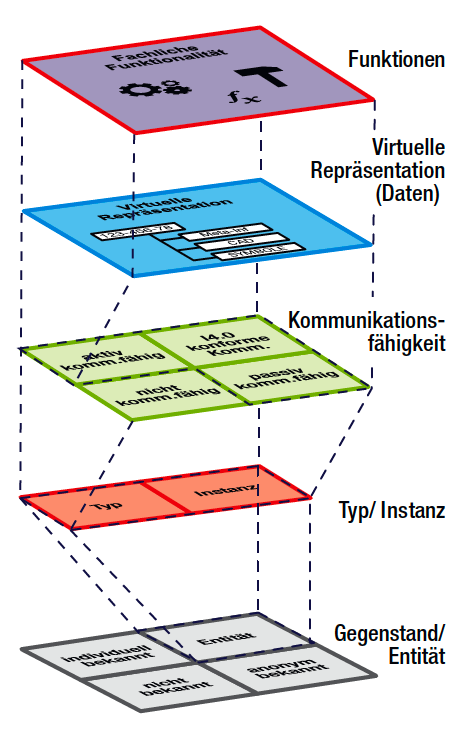
\includegraphics[width=0.5\linewidth]{Ebenen_I40_Kompo.png}
  \caption[Ebenen der Industrie-4.0-Komponente]{Ebenen der Industrie-4.0-Komponente \citep[S. 52]{BITKOM2015}}
  \label{ebenen_i40}
\end{figure}

\subsubsection{Systementwurf gemäß Architekturkonzept}

eigene Architektur aufmalen

